\documentclass[12pt,letter]{article}
% \usepackage[utf8]{inputenc}
\usepackage{graphicx}
\usepackage{amsmath}
\usepackage{amssymb}
\usepackage[left=2cm,right=2cm,top=3cm,bottom=2cm]{geometry}
\usepackage{float}
\usepackage[super,sort&compress,comma]{natbib} \usepackage[font={small}]{caption} %scriptsize = 8pt; footnotesize = 9pt; small = 10pt; normalsize = 11pt (set on line 4 above)
\usepackage[labelfont=bf]{caption}
\usepackage{bm}
\usepackage{dsfont}
\usepackage{pdflscape}
\usepackage[T1]{fontenc}
\usepackage[version=4]{mhchem}
\usepackage{textcomp}
\usepackage{titling}
 \newcommand{\textapprox}{\raisebox{0.5ex}{\texttildelow}}
\usepackage{color}
\include{MyCommand}
\newcommand{\JPH}[1]{{\color{red}{#1}}}
\usepackage{tabularx}
\usepackage{bm}
\usepackage[left]{lineno}
\linenumbers


 \setcounter{figure}{0}
 \let\oldthefigure\thefigure
 \renewcommand{\figurename}{Supplementary Figure}

\renewcommand\refname{Supplementary References}

\begin{document}
\title{Supplementary Information: Title}
\author{Joseph Heindel$^{1,2}$, Teresa Head-Gordon$^{1,2,3}$}
\date{\vspace{-10ex}}
\maketitle
\noindent
\begin{center}
$^1$Kenneth S. Pitzer Theory Center and Department of Chemistry\\
$^2$Chemical Sciences Division, Lawrence Berkeley National Laboratory\\
$^3$Departments of Bioengineering and Chemical and Biomolecular Engineering\\
University of California, Berkeley, CA, USA


corresponding author: thg@berkeley.edu
\end{center}

\newpage
\textbf{Damping function for charge penetration}
The core-shell interactions are damped according to
\begin{equation}
  \bm{T}_{ij}^{damp}=
  \begin{bmatrix}
    1 & \nabla & \nabla^2 \\
  \end{bmatrix}\cdot
  \left(\frac{1}{r_{ij}}f_{ij}^{damp}(r_{ij})\right)
  \label{eq:T_damp}
\end{equation}
\noindent
while the corresponding interaction tensor for shell-shell damping is written as:

\begin{equation}
  \bm{T}_{ij}^{overlap}=
  \begin{bmatrix}
    1 & \nabla & \nabla^2 \\
    \nabla & \nabla^2 & \nabla^3 \\
    \nabla^2 & \nabla^3 & \nabla^4 \\
  \end{bmatrix}\cdot
  \left(\frac{1}{r_{ij}}f_{ij}^{overlap}(r_{ij})\right)
  \label{eq:T_overlap}
\end{equation}
\noindent
The damping functions $f_{ij}^{damp}(r_{ij})$ and $f_{ij}^{overlap}(r_{ij})$ themselves take the following forms.

\begin{subequations}
  \begin{equation}
    f_{ij}^{damp}(r_{ij})=1-\left(1+\frac12b_{j}r_{ij}\right)e^{-b_{j}r_{ij}}
    \label{eq:damp_a}
  \end{equation}
  \begin{equation}
    f_{ij}^{overlap}(r_{ij})=1-\left(1+\frac{11}{16}b_{ij}r_{ij}+\frac{3}{16}(b_{ij}r_{ij})^2+\frac{1}{48}(b_{ij}r_{ij})^3\right)e^{-b_{ij}r_{ij}} 
    \label{eq:damp_b}
  \end{equation}
\end{subequations}
\noindent

The damping function in Eq. \ref{eq:damp_a} can be derived directly from the form
of the Slater density in Eq. \ref{eq:slater} by computing its electrostatic potential.
The damping function in Eq. \ref{eq:damp_b} can be derived from a symmetrized coulomb integral where each
density interacts with the damped potential generated by the other density.\cite{rackers2021polarizable}
Finally, it is important to note that these damping functions are the ones which apply
to charge-charge interactions and that as higher-order multipoles are considered, new damping
functions are generated alongside the gradients of $1/r_{ij}$. In other words, every interaction
tensor in the multipole expansion will be damped differently. We use the same set of damping functions
as derived by Rackers and Ponder which are appropriate for the Slater density in Eq. \ref{eq:slater}.\cite{rackers2021polarizable}
Very similar models have been applied successfully in MB-UCB\cite{das2019development}
based on functional forms proposed by Piquemal\cite{piquemal2003improved} and others\cite{wang2015general,rackers2017optimized}.

\textbf{Environment dependent bonding potential fot the water dimer}
To summarize the large effect this environment-dependent bonding potential has on the forces within FQCT, let us consider a water dimer where each monomer is fixed at the $\omega$B97X-V/def2-QZVPPD geometry. This simply eliminates the geometric distortion forces which are not relevant here. We now compute the forces due to each term in EDA, a so-called force decomposition analysis\cite{aldossary2023force}, and compare them against the same forces predicted by FQCT with and without Eqs. \ref{eq:bond_in_field_2} and \ref{eq:force_constant_in_field_2}.

\begin{table}[ht!]
  \begin{center}
  \begin{tabular}{llcccccc}
      \multicolumn{8}{c}{Water Dimer Force Decomposition Analysis Along \ce{O-H} Bond} \\\hline
       Method & Atom & Mod. Pauli & Cls. Elec. & Disp. & Pol. & CT & Total \\\hline
       FQCT & \ce{O_{don.}}          & -30.1 & 1.4  & 6.0   & -3.4  & -1.5  & -27.5 \\
       No F.D. Morse & \ce{H_{don.}} & -73.7 & 54.5 & 5.3   & 15.4  & 24.9  & 26.4 \\
       & \ce{O_{acc.}}               & 96.4 & -48.9 & -10.1 & -12.7 & -22.3 & 2.4 \\\hline
       FQCT & \ce{O_{don.}} & -15.5 (7.50) & -13.7 & 6.0   & -5.6  & -8.7 & -37.5 \\
       & \ce{H_{don.}}      & -88.5 (-111.9) & 70.0  & 5.3   & 17.7  & 31.9 & 36.4 \\
       & \ce{O_{acc.}}      & 96.4 (95.5)  & -51.7 & -10.1 & -13.0 & -22.0 & -0.4 \\\hline
       $\omega$B97X-V & \ce{O_{don.}} & 3.92 & -15.0  & 0.75  & -8.4  & -15.6 & -34.3 \\
       & \ce{H_{don.}}                & -105.7 & 72.4 & 10.8  & 18.9  & 39.3  & 35.8 \\
       & \ce{O_{acc.}}                & 92.3 & -52.3  & -10.3 & -10.4 & -19.6  & -0.50 \\\hline
  \end{tabular}
  \end{center}
  \caption{Comparison of the forces projected along the \ce{O-H} bond of a water dimer due to each component in the EDA. Forces predicted by FQCT are computed with and without the field-dependent morse potential described in Eqs. \ref{eq:bond_in_field_2} and \ref{eq:force_constant_in_field_2}. The first block of entries is FQCT with no field-dependent Morse potential, the second block is FQCT, and the third is $\omega$B97X-V/def2-QZVPPD. All forces in KJ/mol/\AA. \ce{O_{don.}} and \ce{H_{don.}} are the oxygen and hydrogen atoms donating the hydrogen bond and \ce{O_{acc.}} is the oxygen accepting the hydrogen bond. All forces are projected along the \ce{O-H} bond vector. The numbers in parentheses are what we forces before error fitting with Pauli repulsion.}
  \label{tab:dimer_forces}
\end{table}

The net effect of the field-dependent Morse potential and charge transfer correction is to shift force from the oxygen atom to the hydrogen atom participating in a hydrogen bond. The improvement in accuracy in electrostatics and polarization forces are particularly notable since this correction involves no free parameters. The improvement in Pauli repulsion is also quite large correcting about half the force error at negligible computational cost. The charge transfer forces also remove about half the force error along the \ce{O-H} bond. Note that the Pauli repulsion forces can be quite a bit more accurate with the present model, as shown in the parentheses in Table \ref{tab:dimer_forces}. Since we use the Pauli repulsion to correlate errors in the model, as shown in Figure \ref{fig:error_correlation}, the Pauli forces compensate for remaining errors in the dispersion and charge transfer forces.


In the course of developing this model, we found that we were unable to reproduce the
expected correlation between change in bond length and change in harmonic frequency
for \ce{O-H} stretches.\cite{boyer2019beyond} We ultimately determined that the failure
of our model to reproduce this correlation was due to a lack of coupling between
our bonding potential and the environment. To that end, we extended our Morse potential
to be field-dependent in a manner first described elsewhere.\cite{boyer2019beyond} In short,
the field-dependence of the potential requires specifying the first and second dipole
derivatives along the \ce{O-H} stretch.

Rather than treating these as fitting parameters, we computed the dipole derivatives
from electronic structure as follows. First, we scan along an \ce{O-H} stretch
and compute the total dipole moment, $\mu$, at each point along the scan. This dipole
moment is then projected onto the \ce{O-H} bond vector,
$\mu_{\mathrm{OH}}=\frac{R_{\mathrm{OH}}\cdot \mu}{|R_{\mathrm{OH}}|}$. This allows
us to isolate how the dipole changes as the \ce{O-H} vibrates in a particular environment.

We considered three different environments to see how the dipole derivatives depend on the
local environment and ultimately chose a set of parameters we deemed appropriate for
polarization and one to represent the full system. Remember that in EDA, the polarization
energy represents the response of a molecule to the rest of the environment plus mutual
polarization. To that end, we computed an \ce{O-H} stretch of an isolated \ce{H2O} in
a polarizable continuum described by the COSMO model.\cite{klamt2011cosmo} This resulted
in the dipole surface shown with circles in Fig. \ref{fig:dip_derivatives}. The lines
are fits with a second order polynomial,
$\Delta\mu_{\mathrm{OH}}=\mu_{\mathrm{OH}}^{(1)}\Delta R_{\mathrm{OH}}+\mu_{\mathrm{OH}}^{(2)}\Delta R_{\mathrm{OH}}^2$.
For \ce{H_2O} in a dielectric, we find $\mu_{\mathrm{OH}}^{(1)}=0.345$ and $\mu_{\mathrm{OH}}^{(2)}=0.095$. This
is to be compared to the same values for an isolated \ce{H2O} of $\mu_{\mathrm{OH}}^{(1)}=0.165$ $\mu_{\mathrm{OH}}^{(2)}=-0.012$.
The effect of an environment is, therefore, to promote dissociation to ionic products rather than
radicals which is what the change in sign of $\mu_{\mathrm{OH}}^{(2)}$ implies and to make it easier
to elongate the \ce{O-H} bond which is what the magnitude of $\mu_{\mathrm{OH}}^{(1)}$ means.

Interestingly, when the environment is represented by an actual molecule, as with \ce{(H_2O)_2},
the second dipole derivative increases by a lot and increases even further when when a dielectric
continuum is used. This is seen in the points marked with squares in Fig. \ref{fig:dip_derivatives}.
We attribute this large non-linearity in the dipole surface to the role of charge delocalization,
which makes these parameters suitable for the full potential which includes charge transfer.

A water dimer, however, is not a representative environment for liquid water, or even large
water clusters. To remedy this, we constructed a tetrahedrally coordinated water dimer, \ce{(H2O)_{2+6}}.
The notation \ce{(H2O)_{2+6}} indicates that this is a water dimer solvated by six other water
molecules. The cartesian coordinates are available with the manuscript. When this larger solvation environment
is used, we see a further increase in the dipole derivatives beyond just a water dimer.
The dipole derivatives for the central \ce{O-H} stretch in \ce{(H2O)_{2+6}} are $\mu_{\mathrm{OH}}^{(1)}=1.082$ and
$\mu_{\mathrm{OH}}^{(2)}=1.54$. When these values are used in the model, the
$\Delta\omega$ vs $\Delta R_e$ slope is $\approx -17.1\ \mathrm{cm^{-1}/.001\AA}$ over the same clusters.

 \begin{figure} [H]
    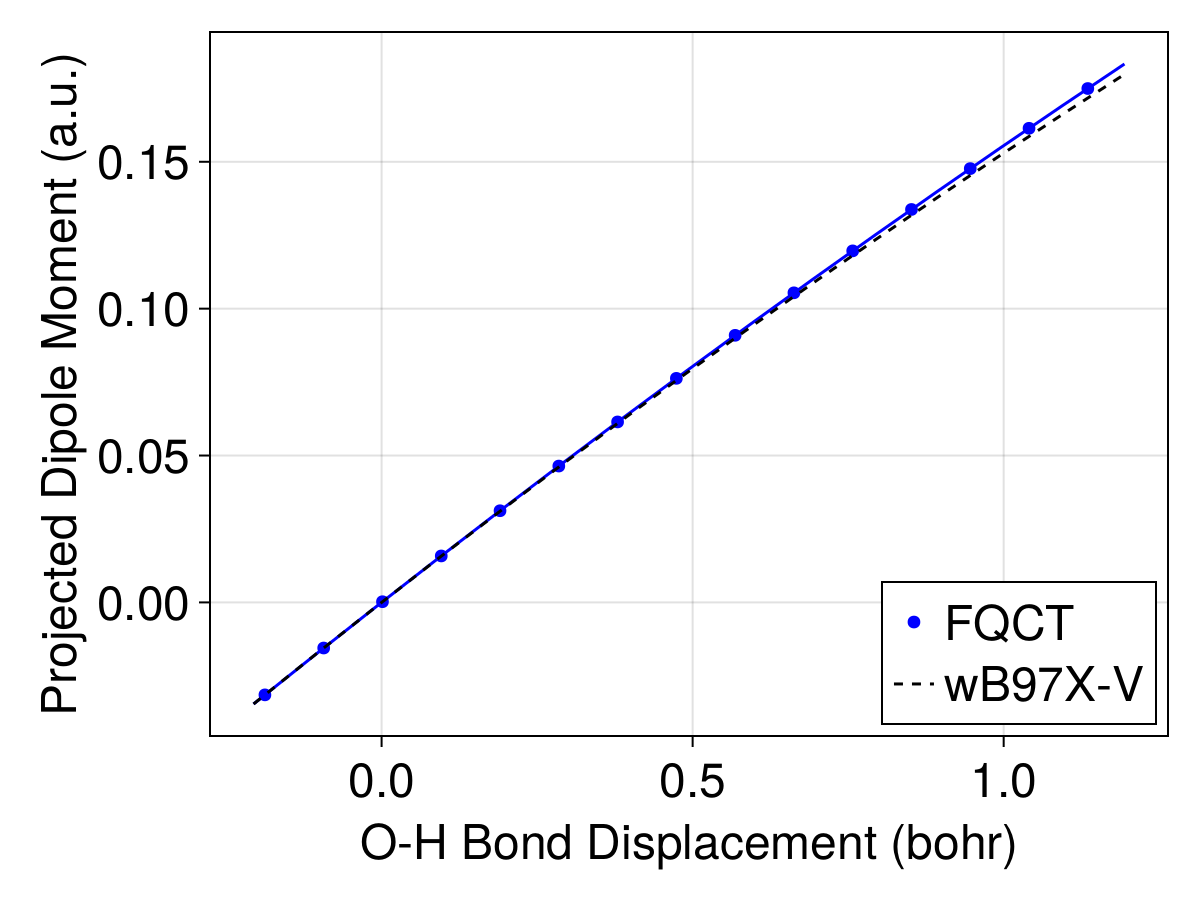
\includegraphics[width=\textwidth]{figures/dipole_derivatives.png}
    \caption{\textit{Projected dipole moments along various O-H stretches.}
    The dipole moment of \ce{(H2O)}, \ce{(H2O)_2}, and \ce{(H2O)_{2+6}} are computed with
    $\omega$B97X-V/def2-QZVPPD as a function of the \ce{O-H} stretch distance. All other degrees of freedom are fixed.
    The dipole moment is projected along the \ce{O-H} stretch unit vector. \ce{(H2O)_{2+6}}
    is a water dimer with six additional water molecules placed so that the water dimer is
    tetrahedrally coordinated. The blue points and lines are gas-phase systems while the
    red points and lines include a polarizable continuum. Each point is connected vertically
    to make it clear they are the same structure but in the presence of a polarizable continuum.
    Circles are used for a single water molecule, squares for a water dimer, and triangles for
    the tetrahedrally solvated water dimer. See text for more details and values of computed dipole derivatives.
}
    \label{fig:dip_derivatives}
\end{figure}

In principle, the curves in Figure \ref{fig:dip_derivatives} should eventually be equal when sufficient
explicit solvent is included in the calculation. Since the dipole derivatives computed from
\ce{(H2O)_{2+6}} are not sufficient to reproduce the Badger correlation, we increase
the dipole derivatives until the appropriate correlation is reproduced. This results in values
of $\mu_{\mathrm{OH}}^{(1)}=1.19$ and $\mu_{\mathrm{OH}}^{(2)}=3.69$.

We have already shown in Figure 5 that our model produces accurate three-body contributions to polarization
and charge transfer for water trimers extracted from ion-water clusters. It is interesting to see, however,
the 2-body and many-body contributions to each component of the energy for whole water clusters. To that end,
we computed the 2-body and many-body contributions for a subset of the reference structures
used in Tables 3 and 4. A comparison of these quantities as computed with $\omega$B97X-V/def2-QZVPPD and FQCT is shown in Table \ref{tab:mbe}.

\begin{landscape}
\begin{table}[ht!]
  \begin{center}
    \begin{tabular}{llcccccccccc}
      \multicolumn{12}{c}{Comparison of Many-Body Expansion for EDA Components (kcal/mol)} \\\hline
      \ce{(H2O)_n}& Component & \multicolumn{2}{c}{Cls. Elec.} & \multicolumn{2}{c}{Mod. Pauli} & \multicolumn{2}{c}{Disp.} & \multicolumn{2}{c}{Pol.} & \multicolumn{2}{c}{CT} \\\hline
      & & FQCT & $\omega$B97X-V & FQCT & $\omega$B97X-V & FQCT & $\omega$B97X-V & FQCT & $\omega$B97X-V & FQCT & $\omega$B97X-V \\\hline
      \ce{(H2O)_3} & 2-Body    & -27.28 & -26.77 & 29.05 & 28.87 &  -6.31  & -6.28  &	-3.38  & -3.48  &	-6.13  & -6.08 \\
             & $\ge$ 3-Body    & -      & -      & 0.0   & -0.24 &   0.0   & 0.21   &	-1.43  & -1.63  &	-0.69  & -0.74 \\\hline
                    & Total    & -27.28 & -26.77 & 29.05 & 28.63 &  -6.31  & -6.07  &	-4.82  & -5.11  &	-6.82  & -6.82 \\\hline
      \ce{(H2O)_6} & 2-Body    & -79.27 & -78.43 & 87.70 & 88.40 &	-19.65 & -19.90 &	-10.53 & -10.94 &	-17.86 & -18.41 \\
      Prism & $\ge$ 3-Body     & -      & -      & 0.0   & -0.62 &	 0.0   & 0.83   &	-6.09  & -6.40  &	-2.71  & -2.80 \\\hline
                    & Total    & -79.27 & -78.43 & 87.70 & 87.78 &	-19.65 & -19.07 &	-16.62 & -17.34 &	-20.57 & -21.21 \\\hline
      \ce{(H2O)_6} & 2-Body    & -79.03 & -78.67 & 89.12 & 90.10 &	-19.13 & -19.36 &	-11.01 & -11.25 &	-19.07 & -19.62 \\
      Cage & $\ge$ 3-Body      & -      & -      & 0.0   & -0.66 &	 0.0   & 0.79   &	-5.99  & -6.26  &	-2.91  & -3.07 \\\hline
                    & Total    & -79.03 & -78.67 & 89.12 & 89.44 &	-19.13 & -18.56 &	-17.00 & -17.51 &	-21.98 & -22.69 \\\hline
      \ce{(H2O)_{10}} & 2-Body & -163.4 & -162.4 & 189.1 & 192.2 &	-37.89 & -38.34 &	-24.16 & -24.92 &	-42.01 & -43.27 \\
                & $\ge$ 3-Body & -      & -      & 0.0   & -0.68 &	0.0    & 1.18   &	-14.24 & -14.92 &	-7.19  & -7.42 \\\hline
                & Total        & -163.4 & -162.4 & 189.1 & 191.5 &	-37.89 & -37.16 &	-38.40 & -39.84 &	-49.20 & -50.69 \\\hline
      \ce{(H2O)_{16}} & 2-Body & -280.5 & -277.7 & 325.0 & 329.0 &	-67.23 & -67.61 &	-41.26 & -42.44 &	-71.59 & -73.15 \\
      Antiboat  & $\ge$ 3-Body & -      & -      & 0.0   & -1.06 &	0.0    & 2.17   &	-25.58 & -27.07 &	-12.05 & -12.37 \\\hline
                & Total        & -280.5 & -277.7 & 325.0 & 327.9 &	-67.23 & -65.44 &	-66.84 & -69.51 &	-83.64 & -85.52 \\\hline
      \ce{(H2O)_{20}} & 2-Body & -358.8 & -355.4 & 416.5 & 420.9 &	-89.17 & -89.20 &	-52.53 & -54.26 &	-91.46 & -92.80 \\
      ES Prism  & $\ge$ 3-Body & -      & -      & 0.0   & -1.66 &	0.0    & 3.03   &	-32.69 & -34.85 &	-15.04 & -15.21 \\\hline
                & Total        & -358.8 & -355.4 & 416.5 & 419.3 &	-89.17 & -86.17 &	-85.22 & -89.11 &	-106.5 & -108.0 \\\hline
    \end{tabular}
  \end{center}
  \vspace{-3mm}
  \caption{Comparison of the 2-body, many-body (i.e. $\ge$ 3-Body), and total energies as predicted by FQCT and as computed with $\omega$B97X-V/def2-QZVPPD.
  Both calculations are done at the \textit{ab initio} optimized geometries. Names of isomers, when applicable, are written below the
  cluster size.
  }
  \label{tab:mbe}
\end{table}
\end{landscape}

One of the significant advantages of using data from EDA to parameterize a
force field is it allows for very fine-grained analysis of the accuracy of a model.
We illustrate this in Table \ref{tab:mbe} by comparing the 2-body, many-body, and total
energies as computed by our force field and $\omega$B97X-V/def2-QZVPPD. First, we can see
that the model is generally very accurate at reproducing each term, as should be expected
given the excellent performance of the model in reproducing total energies and optimized
strcutures. With that being said, there are a couple of apparent shortcomings. First,
we currently do not include many-body dispersion which is very small but not entirely
negligible, especially considering it is the only term besides Pauli repulsion which is
repulsive. It is sometimes argued that many-body dispersion can be ignored since there is
also a small many-body exchange effect which is attractive and hence offsets many-body
dispersion. It is clear from Table \ref{tab:mbe} that this is at least
approximately true in EDA. Even if the cancellation were perfect, however, that does
not guarantee the forces will cancel. For that reason, we may explore adding many-body
dispersion in the future, but neglect it for now since many-body charge transfer
is generally much more important.

Additionally, it is apparent that our model slightly understimates two-body contributions
to both polarization and charge transfer. This likely arises from a limitation of the
functional forms and hence suggests improvements that can be explored in the future.
Our description of many-body contributions to charge transfer, however, are excellent.
Table \ref{tab:mbe} also provides information about ways in which we have gotten lucky
in the parameterization of this model. For instance, in larger clusters the model's dispersion
energies are slightly too attractive while our polarization model is not quite attractive
enough. This cancellation of errors was not intended but likely contributes, in some small
way, to the successes we have seen in Tables 4 and 5.

We are digging into such detail with the hopes that future force fields will do the same.
Electronic structure only used to be able to provide coarse-grained information in the form
of total energies and forces. This hampered the ability to pinpoint limitations of a force field.
Now, however, we can easily identify systematic errors in a force field using the powerful
combination of the many-body expansion and energy decomposition analysis.

Supplementary Table S\ref{tab:mae} presents the mean absolute errors (MAEs) and skewness over each cluster size for each energy category in the EDA. %Focusing on the dimers first, it is clear that the term in error by the most is Pauli repulsion, but even this is in error by less than 0.25 kcal/mol on average. Note that this MAE includes the re-parameterization to maximize error cancellation. Without including error cancellation, the Pauli MAE for dimers is 0.20 kcal/mol and all other terms, besides the interaction energy, remain the same. 
In general, the MAEs obtained by this model are excellent. In addition to the MAEs for each category of the EDA, we also report the skewness of the error distribution. %The skewness is the standardized third moment of a distribution and is a simple measure of asymmetry. Ideally, this number will be zero indicating that the errors are symmetrically distributed. For reference, a skewness between -0.5 and 0.5 is generally interpreted as indicating an approximately symmetric distribution. Therefore, every individual term in our model is very nearly unbiased in the sense of having approximately symmetric errors. The only term of some concern is the interaction energy of dimers which has a skewness of 1.09. Note, however, that the MAE is 0.093 kcal/mol and this asymmetry in the error shrinks as larger clusters are considered. One contributor to the asymmetry in the dimer interaction energies is the lack of many-body dispersion. That is, we have not included many-body dispersion in this model and, as a result, we have to fit the dispersion to implicitly account for this error. This is why the distribution of dispersion errors starts out positively skewed (i.e. too weakly attractive) and ends up negatively skewed (i.e. too attractive). This follows from the fact that many-body dispersion is repulsive on average. It is quite interesting to note that the dimer interaction energy is in error by less than every category besides polarization and dispersion. This immediately indicates that there must be rather significant error cancellation.

\begin{table}[ht!]
  \begin{center}
  \begin{tabular}{lccccc}
      \multicolumn{5}{c}{MAE of Force Field EDA Terms (kcal/mol)} \\\hline
       & \ce{(H2O)2} & \ce{(H2O)3} & \ce{(H2O)4} & \ce{(H2O)5} \\\hline
      %Deform. &  &  &  &  \\
      Pauli (no error fit)   & 0.134 (1.513)  & 0.209 (0.538) & 0.277 (0.491) & 0.329 (0.400) \\
      Pauli                  & 0.184 (0.335)  & 0.297 (0.090) & 0.387 (0.193) & 0.506 (-0.059) \\
      Electrostatics         & 0.125 (-0.209) & 0.205 (0.234) & 0.276 (-0.104) & 0.342 (-0.062) \\
      Dispersion             & 0.069 (0.090)  & 0.092 (-0.124) & 0.109 (-0.407) & 0.149 (-0.420) \\
      Polarization           & 0.046 (-0.219)  & 0.087 (-0.037) & 0.121 (0.437) & 0.154 (0.496) \\
      Charge Transfer        & 0.112 (-0.362)  & 0.168 (-0.342) & 0.229 (-0.116) & 0.269 (-0.118) \\\hline
      Interaction            & 0.093 (1.09) & 0.172 (0.940) & 0.237 (0.330) & 0.298 (0.399) \\\hline
  \end{tabular}
  \end{center}
  \vspace{-3mm}
  \caption{Comparison of the mean absolute error (MAE) in kcal/mol of all terms in the EDA against predictions of our
  water model for hydrogen-bonded water dimers, trimers, tetramers, and pentamers. The numbers in parentheses are
  the skewness of the error distribution.
  In total, there are 2400 each of dimers, trimers, tetramers, and pentamers.
  The first row shows the Pauli repulsion energy without inclusion of error fitting
  while the second row is the Pauli repulsion used in the final model which is calibrated
  to maximize error cancellation.}
  \label{tab:mae}
\end{table}

\bibliographystyle{unsrtnat}
\bibliography{references}
    
\end{document}
